\scanpage{28}
$b)$ La portion de suite exacte
\diagram{\begin{tikzcd}[column sep=small,row sep=small]
H^{2n}(W)\arrow[r,no head]\arrow[d,equals]&H^{2n}(W-W_0)\arrow[r,no head,"\mathrm{inj}"]&H^{2n-1}(W_0)\arrow[r,"\mathrm{surj}"]\arrow[d,equals]&H^{2n+1}(W)\arrow[r,no head]\arrow[d,equals]&H^{2n+1}(W-W_0)\arrow[r,no head]\arrow[d,equals]&H^{2n}(W_0)\arrow[r]\arrow[d,equals]&0\\
0&&\Lambda&&0&0\\[-1em]
&&&\Lambda
\end{tikzcd}}
\margin{si $W_0$ est connexe, tjrs le cas si $n\ge2$}
donne
\[\left\{\begin{gathered}
\boxed{H^{2n}(W-W_0)}=H^{2n+1}(W-W_0)=0\\
\underset{\Vert\;\Lambda}{H^{2n-1}(W_0)}\simeq\underset{\Vert\;\Lambda}{H^{2n+1}(W)}
\end{gathered}\right.\]
\margin{\unsure{conclusion visible de} Lefschetz affine local plus bas}
\margin{\uline{NB} $H^i(W_0)=0$ sauf si $i\in[0,2n-1]$. $H^\bullet(W_0)$ satisfait dualité de Poincaré}
\margin{\deleted{\unsure{supposons}}}
\margin{\uline{NB} $W$ sph. coh. $\Longleftrightarrow$ \deleted{\unsure{\(W-W_0\)}}
\[\left\{\begin{gathered}H^i(W-W_0)\xrightarrow{\sim}H^{i-1}(W_0)\quad\text{si }i\ne0,2n\\
\text{et }H^{2n}(\deleted{W}\unsure{W}-W_0)\hookrightarrow H^{2n-1}(W_0)\end{gathered}\right.\]
[Si \deleted{\unsure{de plus}} $W_0$ connexe, cela équivaut à $H^{2n}(W-W_0)=0$]
Si $n\ge2$, et $W$ non-singulier, il \uuline{f.} que $H^{2n}(W-W_0)=0$, $W_0$ connexe}

\figure{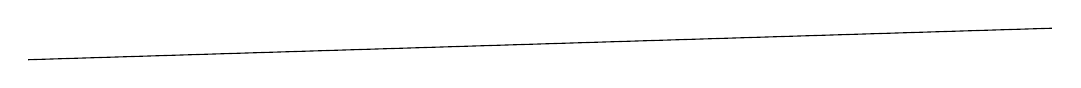
\begin{tikzpicture}\draw (0,0)--(13,0.4);\end{tikzpicture}}
Supposons que $X$ soit régulier en $\deleted{X}x$. Alors on a, par

\uline{Lefschetz local} :
\[\left\{\begin{array}{lll}
H^i(W)\longrightarrow H^i(W_0)&\text{un isom pour}&i\le n-\unsure{2|1}\\
&\text{un mono pour}&i=n\deleted{\unsure{-2}}-1
\end{array}\right.\]
\deleted{Donc si $W$ est une sphère,}

\deleted{Par la suite exacte associée à $e)$, cela signifie}
\inserted{\unsure{dualité cela s'interprète}}
\[\left\{\begin{array}{lll}
H^i_{\unsure{!}}(W_0)\longrightarrow H^{i+2}(W)&\text{un isom si}&i\ge n+\unsure{1}\\
&\text{un épim si}&i\unsure{\ge|=}n\deleted{\unsure{+1}}
\end{array}\right.\]
donc la connaissance de la cohomologie de $W$ implique celle de la cohomologie de $W_0$, sauf en les deux dimensions \deleted{$n-1,n$}\inserted{$H^{n-1}(W_0),H^n(W_0)$} (complémentaires, i.e. où les cohomologies sont duales pour $W_0$).

On peut dire aussi que l'on a
\[\left[\begin{array}{ll}H^i(W-W_0)=0&\text{si }i>n+1\\[-.4em]\quad\Vert&\\[-.4em]\quad H^i(P)&\end{array}\right.\]
\mspage{27}
